\subsection{\Acl{DC}}
\label{ssec:DC}
The idea of \emph{dual algorithms}, to which \acf{DC} belongs, is similar to \ac{MC}. However, instead of generating polygon vertices on the edges of the cubes, this method locates them inside the cubes that have at least one edge which has vertex values both above and below the isovalue (\acs{SignChangingEdge}). The basic algorithm can be summarized in these two steps:
\begin{enumerate}
\item Locate the position of the vertex inside each cube which has at least one \ac{SignChangingEdge}.
\item Join the vertices associated with four cubes sharing a common edge to form a \ac{quad}.
\end{enumerate}
The approach can be seen in \autoref{fig:CompMCDC}, with a similar \ac{MC} illustration for comparison.

\begin{figure}
\begin{center}
\begin{subfigure}{.45\textwidth}
\begin{center}
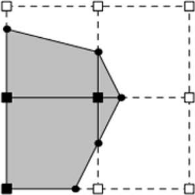
\includegraphics[width=.5\textwidth]{Pictures/SurfaceReconstruction/MC}
\subcaption{\ac{MC} contour}
\label{sfig:MC}
\end{center}
\end{subfigure}
\begin{subfigure}{.45\textwidth}
\begin{center}
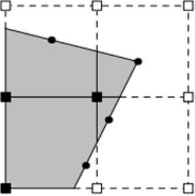
\includegraphics[width=.5\textwidth]{Pictures/SurfaceReconstruction/DC}
\subcaption{\ac{DC} contour}
\label{sfig:DC}
\end{center}
\end{subfigure}
\caption{Comparision of \ac{MC} and \ac{DC} for identical datasets. The vertices are created on the edges of the cubes for \ac{MC} (\autoref{sfig:MC}) and inside the cubes for \ac{DC} (\autoref{sfig:DC}). Please note that the sharp feature in the top right cube can only be reconstructed by \ac{DC}. Figure from \cite{FromVoxelsToPolygons}.}
\label{fig:CompMCDC}
\end{center}
\end{figure}

\begin{comment}
\begin{figure}
\centering
   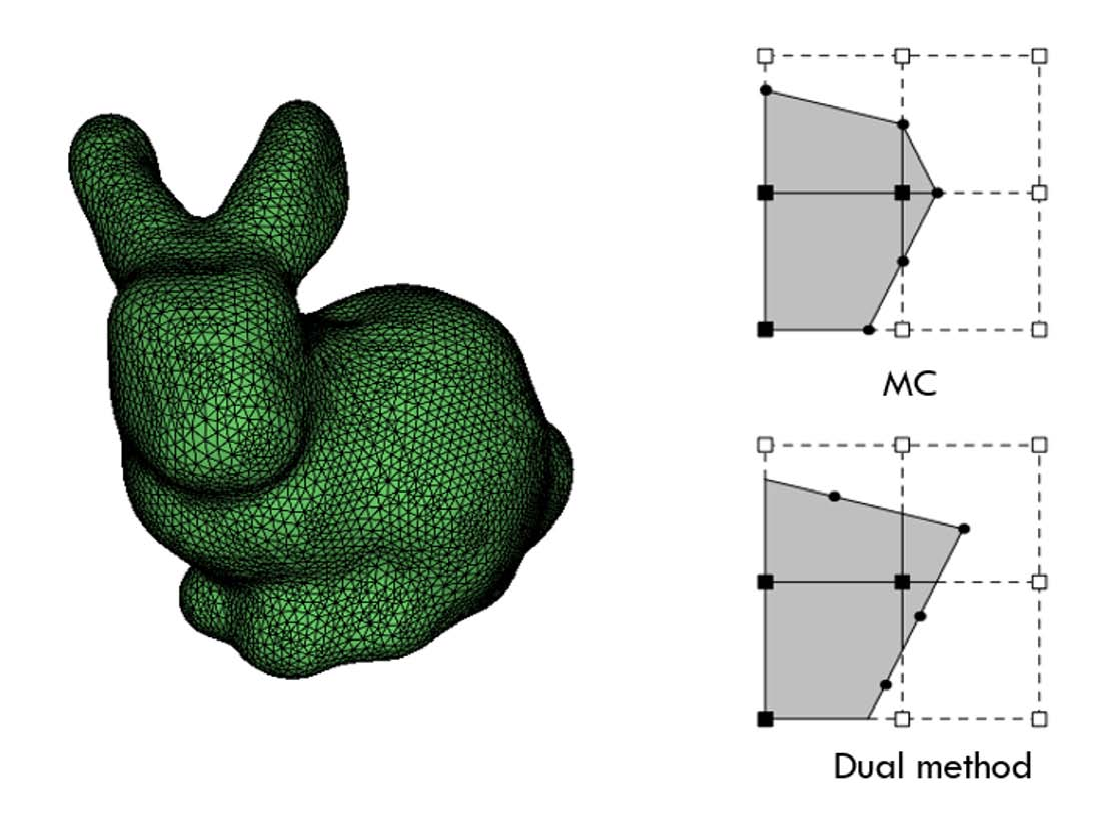
\includegraphics[width=.5\textwidth]{Pictures/bunny_MC.pdf}
   \caption{\textit{Left:} The famous Stanford Bunny, a popular computer graphics test object, here after application of \ac{MC}. \textit{Right:} Main difference between \ac{MC} and \ac{DC}.  Figures taken from \cite{Hermite2002}. }
   \label{fig:bunny_MCDC}
\end{figure}
\end{comment}

\subsubsection{Minimizing the Quadratic Error Function}
Now we want to find out where in the cube the ideal place for the vertex is located, and here different dual algorithms are distinguished. \Ac{DC} in particular generates a vertex positioned at the minimizer of a certain quadratic function. This function depends on the (interpolated) isosurface intersection points, as well as the gradient -- or just the normal of the isosurface -- at these points, both quantities represent the \acs{FirstOrderHermiteData} of the set.
The \acl{QEF} defined in \cite{Hermite2002} is as follows:
\begin{equation}
\label{eq:QEF}
E(x)= x^TA^TAx-2x^TA^Tb+b^Tb
\end{equation}
where the columns of the matrix \textit{A} are the  isosurface normals at the intersection points, and \textit{b} is a vector containing the scalar product of the normals and the intersection points. This system can be solved numerically, for example as proposed in \cite{Hermite2002} by computing the singular value decomposition of \textit{A} and forming the pseudo-inverse, truncating its small singular values. 
The effect of considering the gradient for the calculation of the vertex is huge: \ac{DC} has the ability to represent sharp features like edges and corners.
Computing the position of the new node by just taking the mean value of all the roots on the \acsp{SignChangingEdge} of one cube represent an easier approach, which does not rely on gradient information, but has the disadvantage that it is not able to represent sharp features. The resulting vertex is inside the cube, because it represents the average position of the nodes lying on edges of the cube.

\subsubsection{Non-Manifold Surfaces}
The risk to also obtain non-manifold surfaces represents one of the big drawbacks of \ac{DC}. A manifold surface is defined by the following topological property:
\begin{quote}
\emph{A $d$-dimensional contour is locally a \emph{manifold} if it is topologically equivalent to a $d$-dimensional disc.}\cite{Hermite2002}
\end{quote}
This means that for 2D data we only get a manifold isocontour, if each vertex is connected to exactly 2 edges. For 3D we only get a manifold isosurface, if each edge is at maximum shared by two \acp{quad}. Since the original method does not deal with this issue, extensions have been developed to solve this problem. \autoref{fig:manifold} shows one configuration creating a non-manifold surface for the basic method from \cite{Hermite2002} and its correct resolution by \cite{Schaefer2007}.

\begin{figure}
\begin{center}
\begin{subfigure}[t]{.2\textwidth}
\begin{center}
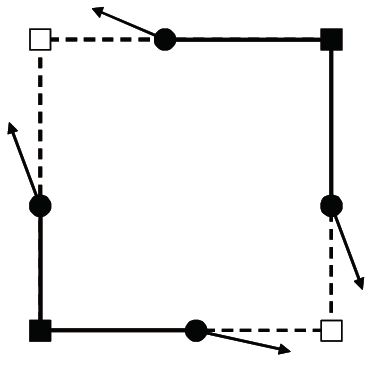
\includegraphics[width=\textwidth]{Pictures/SurfaceReconstruction/ManifoldDC1.png}
\subcaption{Cell with Hermite data}
\label{sfig:ManifoldDC1}
\end{center}
\end{subfigure}
\qquad
\begin{subfigure}[t]{.2\textwidth}
\begin{center}
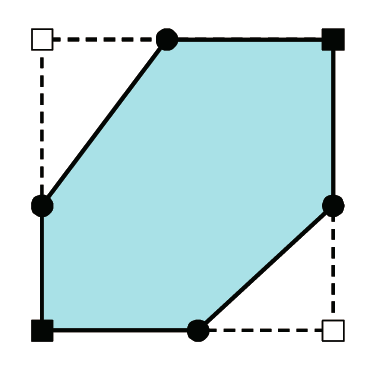
\includegraphics[width=\textwidth]{Pictures/SurfaceReconstruction/ManifoldDC2.png}
\subcaption{manifold contour from \acs{MC}}
\label{sfig:ManifoldDC2}
\end{center}
\end{subfigure}
\qquad
\begin{subfigure}[t]{.2\textwidth}
\begin{center}
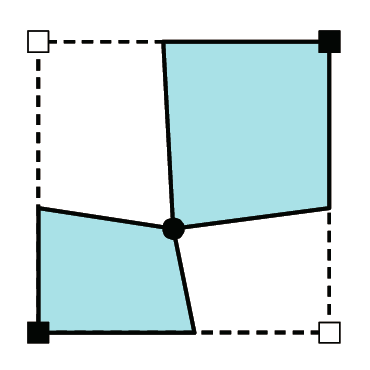
\includegraphics[width=\textwidth]{Pictures/SurfaceReconstruction/ManifoldDC3.png}
\subcaption{non-manifold contour from \acs{DC}}
\label{sfig:ManifoldDC3}
\end{center}
\end{subfigure}
\qquad
\begin{subfigure}[t]{.2\textwidth}
\begin{center}
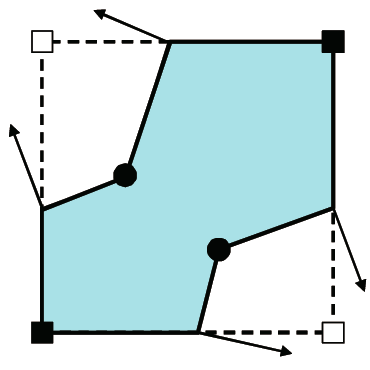
\includegraphics[width=\textwidth]{Pictures/SurfaceReconstruction/ManifoldDC4.png}
\subcaption{manifold contour}
\label{sfig:ManifoldDC4}
\end{center}
\end{subfigure}
\caption{Comparison of contouring for Hermite data \autoref{sfig:ManifoldDC1}. By comparing \autoref{sfig:ManifoldDC2} and \autoref{sfig:ManifoldDC3} one can see that \ac{DC} produces non-manifold surfaces under certain conditions, while \ac{MC} always produces manifold surfaces, but does not incorporate gradient information. Modifying \ac{DC} properly finally gives manifold surfaces in \autoref{sfig:ManifoldDC4}. Figures from \cite{Schaefer2007}}
\label{fig:manifold}
\end{center}
\end{figure}


\begin{comment}
\begin{figure}
\begin{center}
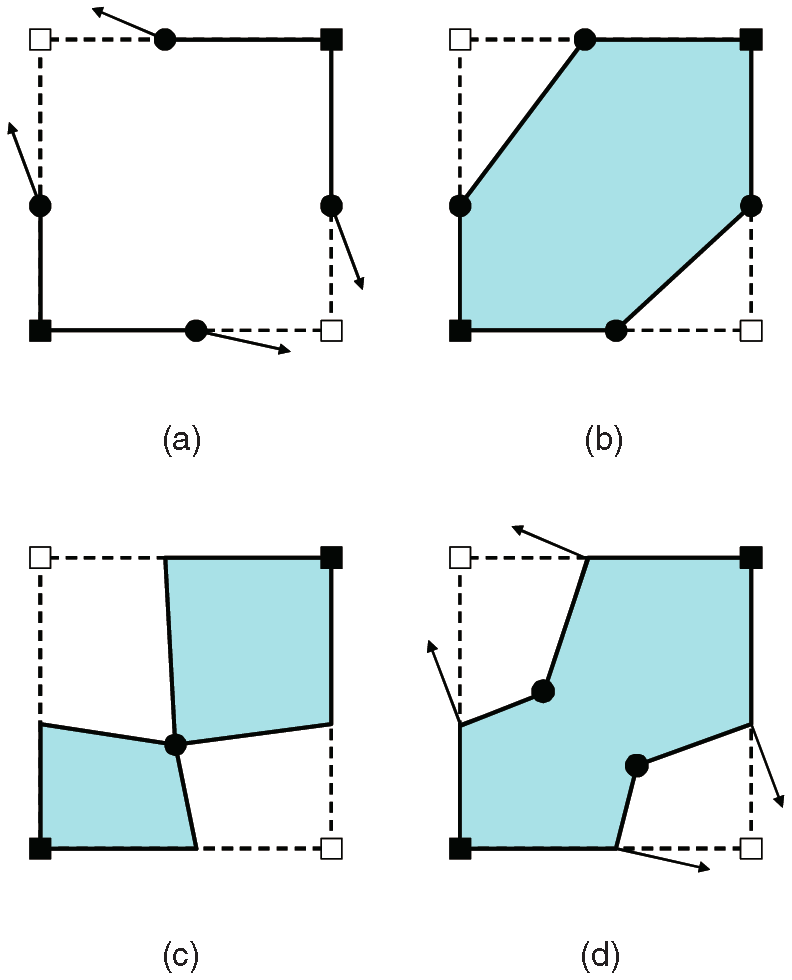
\includegraphics[width=.3 \textwidth]{Pictures/SurfaceReconstruction/ManifoldDC.png}
\end{center}
\caption{Comparison of contouring for Hermite data. (a) Cell with Hermite data on edges, (b) manifold contour from \acs{MC}, (c) non-manifold contour from \acs{DC}, (d) manifold contour from \acs{DualMC} (figure and description from \cite{Schaefer2007})}
\label{fig:manifold}
\end{figure}
\end{comment}

\subsubsection{Topology-Safe Adaptivity}
Usually having as few faces as possible is desirable for reasons like filesize and complexity of the mesh. But in its basic form \ac{DC} is working with uniformly distributed data and introduces vertices on a uniform grid. The reconstructed surface mesh has uniform resolution on the whole area and this results in huge files and a uniformly high resolution, if one wants to resolve fine features of the geometry. As a post processing step one could try to simplify the mesh, but especially for \ac{quad} meshes this is a very demanding -- sometimes even impossible -- task \cite{Puppo2010}.

The solution to this problem is adaptivity. Referring to \cite{Hermite2002} it is possible to implement \ac{DC} in an adaptive and topology-safe way. This means we can simplify the obtained \ac{quad} mesh and therefore reduce the number of \acp{quad} needed to represent the surface, while still conserving the topological structure of our surface.
